\begin{minipage}{.7\linewidth}
	\begin{flushleft}
		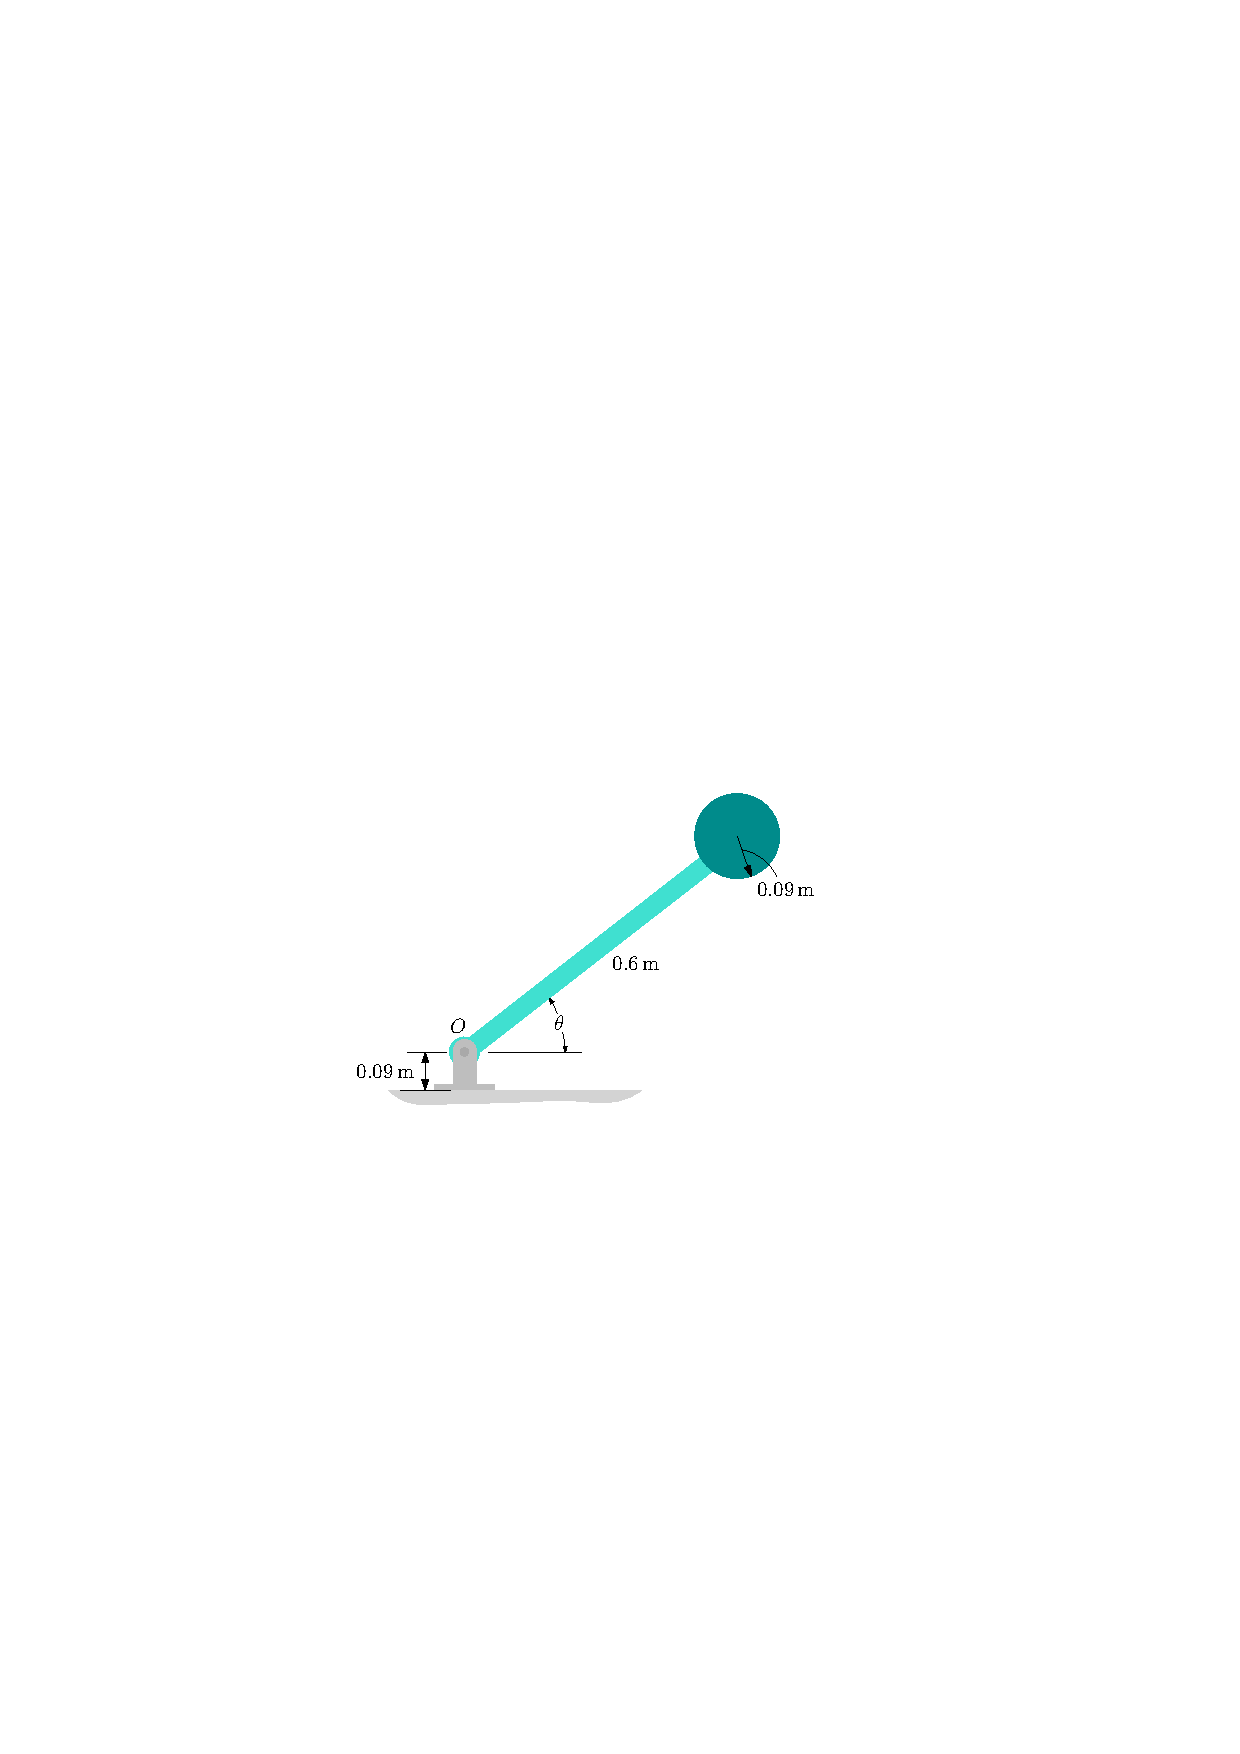
\includegraphics[scale=1.2]{../../images/draw_15}
	\end{flushleft}
\end{minipage}
\begin{minipage}{.3\linewidth}
	\item O pêndulo consiste de uma esfera de \SI{5}{\kilogram} e uma barra de \SI{2}{\kilogram}. Se ele é solto do repouso quando $\theta=90^{\circ}$, determine o ângulo $\theta$ de repique após a esfera bater no chão. Considere $e=0.8$.
	
	\import{../answers}{answer-16}
\end{minipage}